%# -*- coding: utf-8-unix -*-
\chapter{应用二:共模电源抑制比符号化分析}
\label{chap:cmps}

使用第\ref{chap:simp}章中介绍的电路拓扑与双图决策图GPDD之间的关系,可以构造新的GPDD构造方法。
本章中将这种新的构造方法用于运放电路的共模抑制比和电源抑制比分析当中,并利用敏感度分析方法有电路进行调整优化。

\section{双图决策树多端口适用性条件}
\label{sec:cmps:case}

传统的多端口GPDD构造方法会构造一个多根的GPDD结构,并在每个根中生成对应的图对,用于接下来的展开过程\parencite{GShi-GPDD-2013}。
本文则证明了当电路满足一定条件情况下,电路的GPDD构造可以使用一个单根的结构来替代,而不需要多根的展开过程。
这么做的好处主要是可以复用原有的GPDD展开代码,避免了引入新的程序错误,加快了开发效率,减少花费在程序实现上的工作量。

\begin{figure}[!htp]
	\centering
	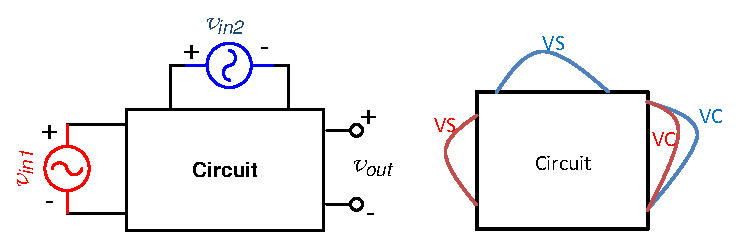
\includegraphics[width=0.8\textwidth]{chap4/MultiPort.eps}
	\bicaption[fig:mp]{多端口电路示意}{多端口电路示意}{Fig}{Multi-Port circuit example}
\end{figure}

假设我们考虑如图\ref{fig:mp}左侧所示的电路结构。
这里电路总共有两个输入端口,而且两个输入端口共享同一个电路输出端口。
将这样的电路结构画成如图\ref{fig:mp}右侧的图,可以看到在输出端口有两条并联的VC边。
由于GPDD算法是对电路中生成树对的枚举过程,所以如果两条VC同时出现在最终的生成树对中,则会形成环路。
所以如图\ref{fig:mpgpdd},必然不会出现两个输入对以实线边相连的情况。

\begin{figure}[!htp]
	\centering
	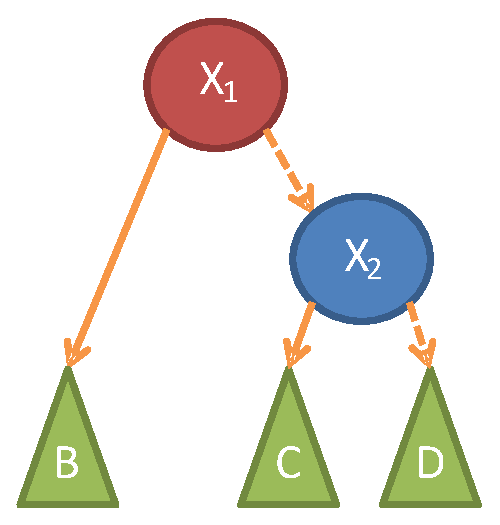
\includegraphics[width=0.3\textwidth]{chap4/MultiPortGPDD.eps}
	\bicaption[fig:mpgpdd]{多端口电路的GPDD结构}{多端口电路的GPDD结构}{Fig}{GPDD structure for multi-port circuit example}
\end{figure}

这里我们用符号$X_1$和$X_2$代表两组输入输出关系。如需要对电路传输函数进行计算,根据第\ref{chap:simp}章中介绍的元件拓扑结构与GPDD之间的关系,我们可以发现某个传输函数即是在另一个输入输出对符号置零情况下得到的结果。区别于之前章节的记号,这里使用比较简单易写的$f\left( N \right)$来作为节点$N$的GPDD计算结果。所以可以根据下两式对电路的传输函数进行计算:

\begin{eqnarray}
{H_1}\left( s \right) = \frac{{{v_{out}}}}
{{{v_{in1}}}} = \frac{1}
{{{X_1}}} = \frac{{f\left( B \right)}}
{{f\left( D \right)}} \hfill \\
{H_2}\left( s \right) = \frac{{{v_{out}}}}
{{{v_{in2}}}} = \frac{1}
{{{X_2}}} = \frac{{f\left( C \right)}}
{{f\left( D \right)}} \hfill 
\end{eqnarray}

另外可以看到电路传输函数共享同一个分母,这与基本电路两端口的性质是一致的。
只要在满足如下定理的情况下,这种情况在推广到更多的端口与更大的电路规模仍然成立。

\begin{thm}\label{thm:mpcon}
	在满足以下条件之一的情况下,GPDD可以用单根构造的方式构造多端口电路,且不会出现多个输入输出端口符号的交叉项:
	\begin{enumerate}[label=\emph{\alph*})]
		\item 所有端口的输出端均在同一端口测量同种信号(电流或电压)。
		\item 所有端口的输入端均在同一端口施加同种信号(电流或电压)。
	\end{enumerate}
\end{thm}

这里使用生成树对枚举的方式对定理的正确给出说明,解析化的证明方式在附录\ref{app:mpcon} 中给出。
我们只对输出端可能出现的$VC$边和$CC$边进行说明,输入端的$VS$和$CS$可以类比得到。

首先来考虑VC边,我们知道,对同一个端口的电压进行测量,那么相应的所有的$VC$边必然并联。
那么很明显如果有多个$VC$被包含的情况下,必然形成环,不会出现树的结构,故生成的GPDD中必然不含有有多个输入输出端口符号的符号化项。
其次我们考虑CC边,对同一个端口的电流进行测量,那么相应的所有的$CC$边必然串联。
根据GPDD理论\parencite{GShi-GPDD},如需符号项需包含有CC边的符号,那么在生成树对中的左树中CC边并不会包含在最终的树中。
由于,$CC$边串联,故如有两个或以上输入输出符号被包含在符号项中时,必然造成图中出现了分离的图,而分离的图无法生成树结构。
这样的话我们就可以得到定理\ref{thm:mpcon}的条件a,条件b可以用类似的方法说明。

\section{用于共模抑制比与电源抑制比分析}
\label{sec:cmps:cmrrpsrr}

\subsection{共模抑制比与电源抑制比介绍}
\label{subsec:cmps:cmrrpsrr:intro}

运算放大器除了差分增益响应以及相对应的相位变化,别的设计指标也是极为关键的。
在近几年兴起的生物电路中,由于生物电信号的较为微弱的特性,共模及电源噪声信号的影响对相关的运算放大器设计工作提出了很高的要求\parencite{Sawan-CMRR-1999,Abdullah-Biopotential-2015,Paul-22dBPSRR-2012}。
目前对这两方面指标的自动化辅助工具的研究比较欠缺,故十分需要有相应的工具对此种类型的电路分析工作进行指导与辅助。

根据\parencite{GRAY-Analog}中的定义,可根据图\ref{fig:cmps}中的示意给出共模抑制比(Common Mode Rejection Ratio, $CMRR$)和电源抑制比(Power Supply Rejection Ratio, $PSRR$)的定义。

\begin{figure}[!htp]
	\centering
	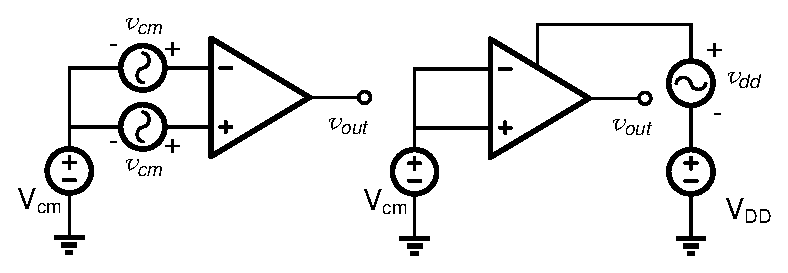
\includegraphics[width=0.8\textwidth]{chap4/CMPS.eps}
	\bicaption[fig:cmps]{共模抑制比及电源抑制比定义}{共模抑制比及电源抑制比定义}{Fig}{CMRR and PSRR definition}
\end{figure}

首先给出CMRR的定义,如图\ref{fig:cmps}左侧所示,一个差分运算放大器有两个差分输入端,如果在两个输入端输入叠加在共模信号上的差分信号。
用$v_d$和$v_{cm}$代表信号的差模和共模部分,那么我们可以得到运放的输出信号的差模部分有$v_{out}^{d} = A_v v_d$;而共模输出信号有$v_{out}^{cm} = A_{cm} v_{cm}$。
这里$A_v$和$A_{cm}$代表了运放的差模和共模增益。那么可以将CMRR定义为差模增益与共模增益的比值,如下式所示。

\begin{equation}
CMRR = \left|\frac{A_v}{A_{cm}}\right|
\end{equation}

接着给出PSRR的定义,如图\ref{fig:cmps}右侧所示,运放的电源电压部分给上一个小信号激励$v_{dd}$。
那么运放输出中由电源处提供的信号可以表示为$v_{out}^{ps} = A_{ps}v_{dd}$,这里$A_{ps}$代表了运放的电源增益。
故可以将PSRR定义为差模增益与电源增益的比值,如下式所示。

\begin{equation}
PSRR = \left|\frac{A_v}{A_{ps}}\right|
\end{equation}

可以看到运放的CMRR和PSRR均是通过小信号计算得到,故可以使用符号化分析得到相应的结果。
同时可以看到在分析CMRR和PSRR的过程中用到3个增益:$A_v$、$A_{cm}$和$A_{ps}$。
这三者的输出端均为测量电压,且为同一个端口的测量,故满足上一节所给出的定理\ref{thm:mpcon},那么可以使用单根的GPDD多端口的符号化分析方法对CMRR和PSRR进行分析。

\subsection{双图决策树多端口计算方法}
\label{subsec:cmps:cmrrpsrr:cal}

CMRR和PSRR的分析总共涉及3个输入输出对:

\begin{enumerate}
	\item 差分输入到输出端的差模电压增益$A_v$
	\item 共模噪声到输出端的共模电压增益$A_{cm}$
	\item 电源扰动到输出端的电源电压增益$A_{ps}$
\end{enumerate}

这三组输入输出对对应了不同的输入信号端口。
因此在符号化构建的过程中,我们只需要在输入网表顶部给出3组VCVS的受控源,即可完成符号化网表的构建。
这三组受控源这里分别用$X_v$、$X_{cm}$和$X_{ps}$三个符号给出,经过多端口符号化构造过程,可以得到类似于图\ref{fig:cmpsgpdd}的GPDD结构。

\begin{figure}[!htp]
	\centering
	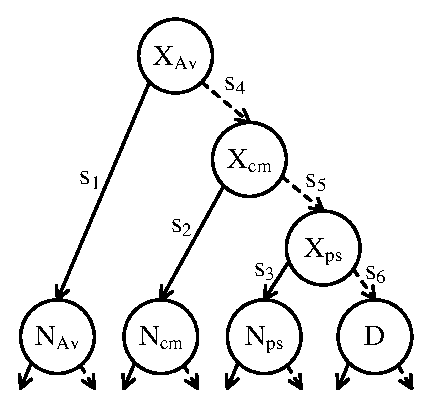
\includegraphics[width=0.35\textwidth]{chap4/CMPSGPDD.eps}
	\bicaption[fig:cmpsgpdd]{多端口方法构造CMRR及PSRR的GPDD结构}{多端口方法构造CMRR及PSRR的GPDD结构}{Fig}{GPDD Structure for multi-port construction of CMRR and PSRR}
\end{figure}

这里的子GPDD结构由$N_{Av}$,$N_{cm}$,$N_{ps}$和$D$这四个GPDD节点为根组成。
我们将使用他们的符号化结果来计算得到CMRR和PSRR的值。
那么根据GPDD的求值规则,辅以符号化电路元件约减的性质,可以得到之前的三个增益可用下式计算得到。

\begin{eqnarray}
A_v     &= \frac{1}{X_{Av}} &= - s_1 s_4 s_5 s_6 \frac{f\left(N_{Av}\right)}{f\left(D\right)}\\
A_{cm}  &= \frac{1}{X_{cm}} &= - s_2 s_5 s_6 \frac{f\left(N_{cm}\right)}{f\left(D\right)}\\
A_{ps}  &= \frac{1}{X_{ps}} &= - s_3 s_6 \frac{f\left(N_{ps}\right)}{f\left(D\right)}
\end{eqnarray}

同时,根据CMRR和PSRR的定义,可以简化CMRR和PSRR在GPDD中的计算如下:

\begin{eqnarray}
CMRR &=& s_1 s_2 s_4 \frac{f\left(N_{Av}\right)}{f\left(N_{cm}\right)}\\
PSRR &=& s_1 s_3 s_4 s_5 \frac{f\left(N_{Av}\right)}{f\left(N_{ps}\right)}
\end{eqnarray}

值得注意的是,这里GPDD的构造过程只需要一次。
只要知道所有电路符号元件的值,而后$A_v$,$CMRR$和$PSRR$的数值结果可以通过自底向上遍历GPDD结构同时得到,节省了计算时间。
这样的计算效率在之前提出的一些符号化方法中是不可行的\parencite{Gielen-ISAAC-1989}。

\section{符号化敏感度分析方法}
\label{sec:cmps:sens}

GPDD理论中关于电路的敏感度分析将大大有助于模拟电路工程师加深对电路设计的理解,帮助电路工程师对电路性能优化提供更多的具有洞察力的信息\parencite{MengXiaoxuan-Sens-2009,WengBinbin-Sens-2011,ChenJiajun-Sens-2012}。

这里对符号化敏感度分析做一定回顾,并给出考虑CMRR和PSRR特殊情况下的计算规则。敏感度定义如下:

\begin{equation}
Sens\left( {H\left( s \right),p} \right) = \mathop {\lim }\limits_{\Delta p \to \infty } \left\{ {\frac{{\frac{{\Delta H\left( s \right)}}{{H\left( s \right)}}}}{{\frac{{\Delta p}}{p}}}} \right\} = \frac{p}{{H\left( s \right)}}\frac{{\partial H\left( s \right)}}{{\partial p}}
\end{equation}

敏感度反应了电路传输函数$H\left(s\right)$的变化对参数$p$的变化的所产生的影响。
可以想象若敏感度绝对值很高,则$p$的变化会引起较大的数$H\left(s\right)$的改变。若我们选择各个MOS晶体管的宽$W$为$p$,那么就可以求得电路元件尺寸与电路性能直接关系,则可以得到如下公式。

\begin{equation}\label{eq:DCSens}
Sens\left( {H\left( s \right),{W_i}} \right) = \frac{{{W_i}}}{{H\left( s \right)}} \sum\limits_{j} \sum\limits_{p} {\frac{{\partial H\left( s \right)}}{{\partial {g_{j,p}}}}\frac{{\partial {g_{j,p}}}}{{\partial {W_i}}}}
\end{equation}

其中$W_i$为电路中$i$号MOS管的宽,而$g_{ij}$则为i号MOS管的第j个小信号参数,如:$g_m$,$g_{ds}$,$g_{mb}$,$c_{gs}$等。
可以看到,若我们忽略别的晶体管对$i$号晶体管小信号参数的影响,则上述公式最右侧的式子中H(s)可以由GPDD进行计算,而第二个偏导数可以由器件模型以及DC偏置点决定。
我们通过一个例子来进一步解释式\ref{eq:DCSens}的意义。

\begin{exmp}
运放中的敏感度公式意义

\begin{figure}[!htp]
	\centering
	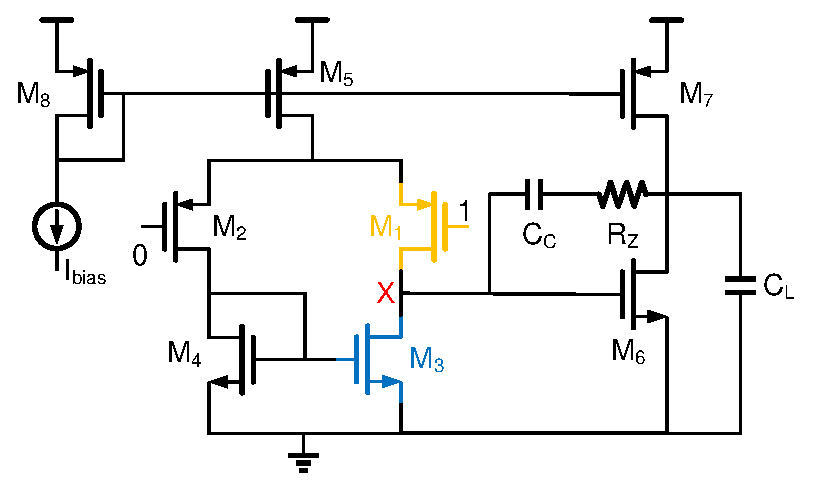
\includegraphics[width=0.7\textwidth]{chap4/TSExample.eps}
	\bicaption[fig:tsexample]{用于敏感度说明的两级运放电路}{用于敏感度说明的两级运放电路}{Fig}{Two-stage opamp for sensitivity explanation}
\end{figure}

考虑图\ref{fig:tsexample}中的运放电路,如果我们需要对这里的$M_1$管的宽$W_1$进行敏感度分析。
根据式\ref{eq:DCSens}中所示,可以得到如下的推导:

\begin{align}
Sens\left( {H\left( s \right),{W_1}} \right) &= \frac{{{W_1}}}
{{H\left( s \right)}}\frac{{\partial H\left( s \right)}}
{{\partial {W_1}}} \nonumber \\ 
&= \frac{{{W_1}}}
{{H\left( s \right)}}\left( {\sum\limits_p {\frac{{\partial H\left( s \right)}}
		{{\partial {g_{1,p}}}}\frac{{\partial {g_{1,p}}}}
		{{\partial {W_1}}}}  + \sum\limits_{j \ne 1,p} {\frac{{\partial H\left( s \right)}}
		{{\partial {g_{j,p}}}}\frac{{\partial {g_{j,p}}}}
		{{\partial {W_1}}}} } \right) \nonumber \\ 
&= \frac{{{W_1}}}
{{H\left( s \right)}}\left( {\frac{{\partial H\left( s \right)}}
	{{\partial {\textcolor{orange}{g_{m1}}}}}\frac{{\partial {\textcolor{orange}{g_{m1}}}}}
	{{\partial {W_1}}} +  \cdots  + \frac{{\partial H\left( s \right)}}
	{{\partial {\textcolor{blue}{g_{ds3}}}}}\frac{{\partial {\textcolor{blue}{g_{ds3}}}}}
	{{\partial {\textcolor{red}{V_X}}}}\frac{{\partial {\textcolor{red}{V_X}}}}
	{{\partial {W_1}}} +  \cdots } \right)
\end{align}

可以看到在最后一步中展开的两项中,其中第一项仅与$M_1$管的参数有关,而第二项还与$M_3$管有关。
造成这种现象的原因主要在于当改变$W_1$的时候,必然会对$X$节点的电压造成影响,故会影响$M_3$管偏置情况,故此时可与$M_3$管中的小信号参数相关。

\end{exmp}

关于式\ref{eq:DCSens}第一项偏导数的计算,其实十分类似我们选取元件取值为无穷大是的计算过程,首先我们假设$H\left(s\right)$的公式如下式所示:

\begin{equation}
H\left( s \right) = \frac{{N\left( s \right)}}{{D\left( s \right)}} = \frac{{{N_1}\left( s \right)Y + {N_2}\left( s \right)}}{{{D_1}\left( s \right)Y + {D_2}\left( s \right)}}
\end{equation}

我们知道线性电路的传输函数一定是一个有理多项分式。
故分子$N\left(s\right)$和分母$D\left(s\right)$均为乘积项之和(Sum of Products,SOP)的形式,且显然分别为GPDD根节点的左右子结构。
$Y$是电路中某个元件的导纳值或者受控源的系数。
显然,我们可以将$N\left(s\right)$和$D\left(s\right)$分解为不包含$Y$这一项的$N_1\left(s\right)$、$N_2\left(s\right)$、$D_1\left(s\right)$和$D_2\left(s\right)$四个式子。
可以注意到由于GPDD结构节点求值的方法,每个节点总是乘以左边的节点的值并加上右边节点的值。
故可以想到$N_1\left(s\right)$是GPDD根节点左侧子结构中忽略所有Y节点的右边连接关系得到的结果,以此类推,可以得到$N_2\left(s\right)$、$D_1\left(s\right)$和$D_2\left(s\right)$相应在GPDD中对应的结构。
对于求取偏导数,我们有

\begin{equation}
\frac{{\partial H\left( s \right)}}
{{\partial Y}} = \frac{{\frac{{\partial N\left( s \right)}}
		{{\partial Y}}D\left( s \right) - N\left( s \right)\frac{{\partial D\left( s \right)}}
		{{\partial Y}}}}
{{{D^2}\left( s \right)}} = \frac{{{N_1}\left( s \right)D\left( s \right) - N\left( s \right){D_1}\left( s \right)}}
{{{D^2}\left( s \right)}}
\end{equation}

上式表示传输函数针对某个电路元件Y的偏导数与$N\left(s\right)$,$D\left(s\right)$,$N_1\left(s\right)$和$D_1\left(s\right)$有关。
可以注意到仅有与$Y$相乘的项得到了保留,相对应的在GPDD中,即仅有与$Y$节点的左边节点才计入计算,右边节点则忽略,这与求取元件无穷大取值情况下的GPDD计算是一致的。
同样的,同时需要注意到由于GPDD的共享性质,有些从根节点到1结点的路径不会经过Y节点,这种项也不能计入其中。

通过简单的推导即可知道,CMRR和PSRR的敏感度也可以通过如下的计算得到:

\begin{equation}
Sens\left( {{CMRR},{W_i}} \right) = Sens\left( {{A_{v}},{W_i}} \right) - Sens\left( {{A_{cm}},{W_i}} \right)
\end{equation}

\begin{equation}
Sens\left( {{PSRR},{W_i}} \right) = Sens\left( {{A_{v}},{W_i}} \right) - Sens\left( {{A_{ps}},{W_i}} \right)
\end{equation}

这意味着我们需要求得三个增益的敏感度,即可得到CMRR和PSRR的敏感度。
同时,由于所有的计算均在同一个GPDD上进行,所以可以高效地求得相应的结果。

\section{共模抑制比与电源抑制比测试结果}
\label{sec:cmps:test}

\subsection{多端口构造方法的双图决策图的时间空间复杂度比较}
\label{subsec:cmps:test:scale}

这里的测试电路选用了图\ref{fig:two_stage}和图\ref{fig:folded_cascode}中的折叠共源共栅运放和两级运放结构。

\begin{figure}[!htp]
	\centering
	\includegraphics[width=0.7\textwidth]{chap4/res/TSRes.eps}
	\bicaption[fig:trres]{两级运放的$CMRR$及$PSRR$的频率响应结果}{两级运放的$CMRR$及$PSRR$的频率响应结果}{Fig}{Frequency response for $CMRR$ and $PSRR$ in two-stage opamp}
\end{figure}

\begin{figure}[!htp]
	\centering
	\includegraphics[width=0.7\textwidth]{chap4/res/FDRes.eps}
	\bicaption[fig:fcres]{折叠共源共栅运放的$CMRR$及$PSRR$的频率响应结果}{折叠共源共栅运放的$CMRR$及$PSRR$的频率响应结果}{Fig}{Frequency response for $CMRR$ and $PSRR$ in folded-cascode opamp}
\end{figure}

相应的小信号电路元件参数通过HSPICE的数值仿真结果得到,并构建相应的GPDD结构。
计算得到的CMRR和PSRR的频率响应曲线在图\ref{fig:trres}和图\ref{fig:fcres}中展示。
可以看到仿真结构与HSPICE的数值结果十分吻合,所以GPDD符号化计算的结果是有效的。

\begin{table}[!htp]
	\bicaption[tab:tscmpsgpdd]{两级运放的单独构造与多端口构造的时空性能比较}{两级运放的单独构造与多端口构造的时空性能比较}{Table}{Comparison between separated and multi-port constructions for the two-stage opamp}
	\centering
	\begin{tabular}{*{3}{c}}
		\hline
		       情况         & $|\mbox{GPDD}|$ & 构造时间 ($\mu s$) \\ \hline
		 单独构造$A_v$的GPDD   &      2251       &     522.0      \\
		单独构造$A_{cm}$的GPDD &      2615       &     408.7      \\
		单独构造$A_{ps}$的GPDD &      3933       &     632.0      \\
		       总计         &      8799       &     1562.7     \\ \hline
		    多端口构造GPDD     &      4871       &     730.1      \\ \hline
		      改进程度        &     44.6\%      &      2.1x      \\ \hline
	\end{tabular}
\end{table}

\begin{table}[!htp]
	\bicaption[tab:fccmpsgpdd]{折叠共源共栅运放的单独构造与多端口构造的时空性能比较}{两级运放的单独构造与多端口构造的时空性能比较}{Table}{Comparison between separated and multi-port constructions for the folded-cascode opamp}
	\centering
	\begin{tabular}{*{3}{c}}
		\hline
		       情况         & $|\mbox{GPDD}|$ & 构造时间 ($s$) \\ \hline
		 单独构造$A_v$的GPDD   &      24228      &   155.2    \\
		单独构造$A_{cm}$的GPDD &      25706      &   122.0    \\
		单独构造$A_{ps}$的GPDD &      32918      &   173.6    \\
		       总计         &      82852      &   450.8    \\ \hline
		    多端口构造GPDD     &      35424      &    78.7    \\ \hline
		      改进程度        &     57.2\%      &    5.7x    \\ \hline
	\end{tabular}
\end{table}

我们也统计我们的软件实现性能来证明多端口构造得到的GPDD共享结果的优势。
首先,我们针对三种增益$A_v$,$A_{cm}$和$A_{ps}$分别单独构造GPDD结构,并统计相应的构造时间和GPDD节点个数。
其相应的结果在表\ref{tab:tscmpsgpdd}和表\ref{tab:fccmpsgpdd}中展现。
总计一栏将上述三个增益分别的表现进行了求和,反映分别构造总复杂度。
然后采用多端口方式构造同时对三个增益构造GPDD。
从表中的数据可以明显地看到多端口电路构造方式的优势,利用更少的时间和更少的计算空间完成了整体的计算。

\subsection{两级运放的电路的参数扫描结果}
\label{subsec:cmps:test:MC}

由于符号化一次构造,多次计算的优良性质,符号化计算可以快速地对电路的参数进行扫描,并从中观察电路元件取值对电路性能的影响。
这里我们对两级运放的补偿部分的两个电路元件补偿电容$C_c$和调零电阻$R_z$进行参数扫描,以观察CMRR和PSRR与其之间的关系。

\begin{figure}[!htp]
	\centering
	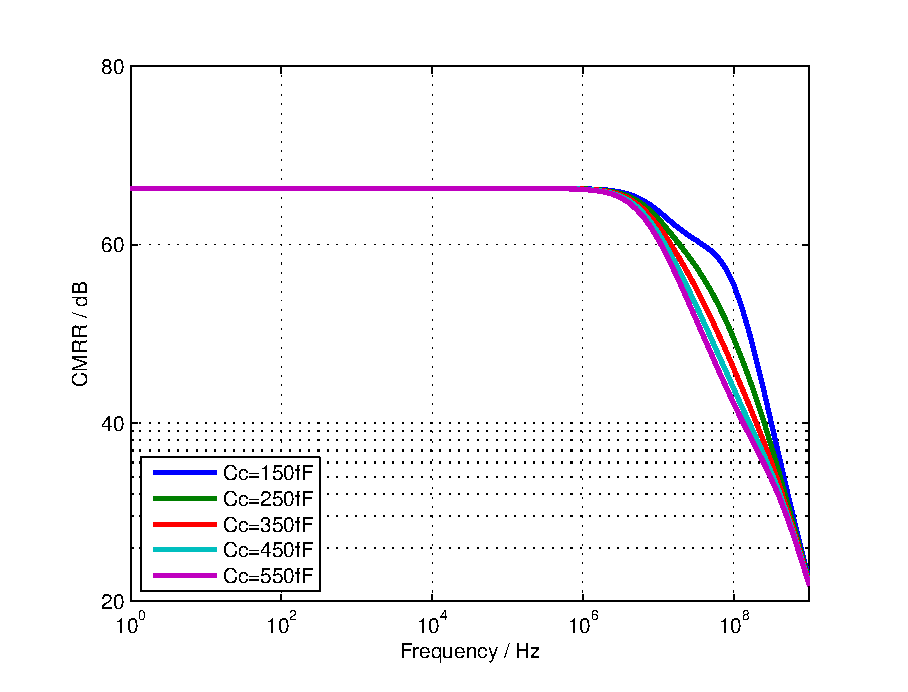
\includegraphics[width=0.7\textwidth]{chap4/res/CMRR_CC.eps}
	\bicaption[fig:cmrrcc]{两级运放针的$CMRR$对补偿电容$C_c$的参数扫描结果}{两级运放针的$CMRR$对补偿电容$C_c$的参数扫描结果}{Fig}{Parameter sweep results for $CMRR$ of compensation capacitor $C_c$ in two-stage opamp}
\end{figure}

\begin{figure}[!htp]
	\centering
	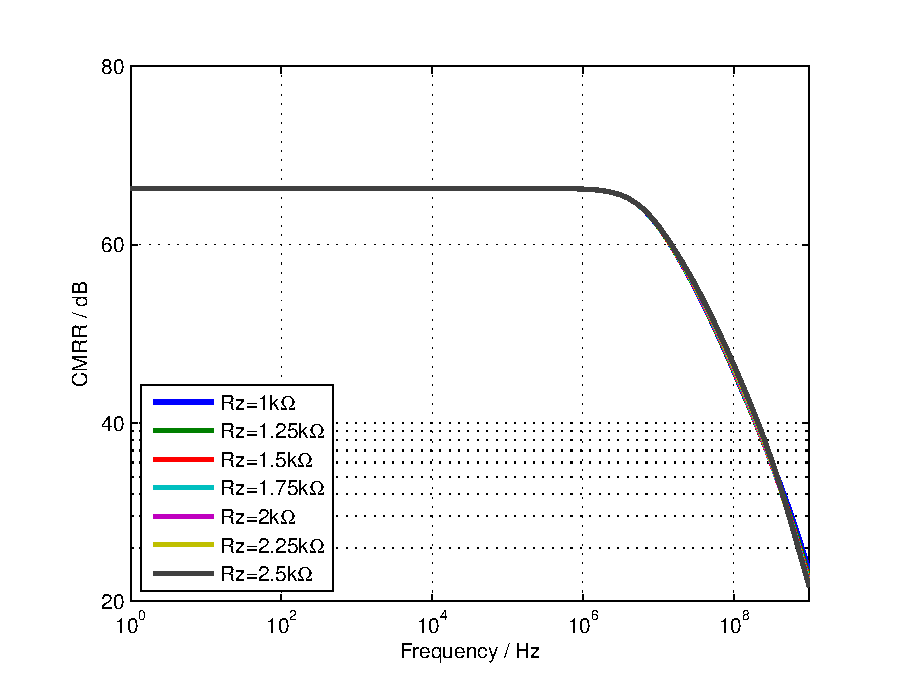
\includegraphics[width=0.7\textwidth]{chap4/res/CMRR_Rz.eps}
	\bicaption[fig:cmrrrz]{两级运放针的$PSRR$对调零电阻$R_z$的参数扫描结果}{两级运放针的$CMRR$对补偿电容$R_z$的参数扫描结果}{Fig}{Parameter sweep results for $CMRR$ of compensation capacitor $R_z$ in two-stage opamp}
\end{figure}

\begin{figure}[!htp]
	\centering
	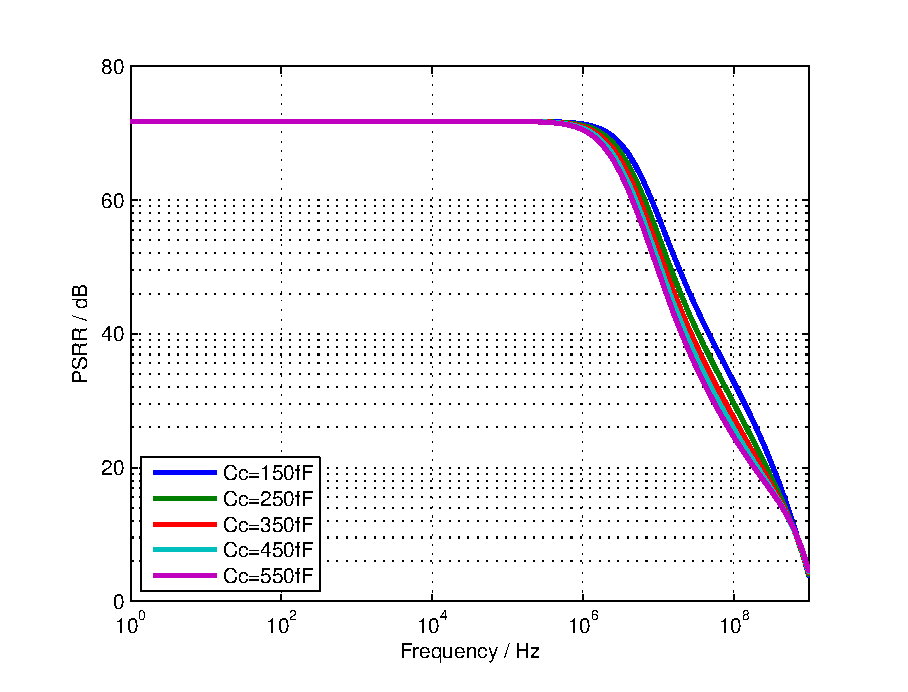
\includegraphics[width=0.7\textwidth]{chap4/res/PSRR_CC.eps}
	\bicaption[fig:psrrcc]{两级运放针的$PSRR$对补偿电容$C_c$的参数扫描结果}{两级运放针的$PSRR$对补偿电容$C_c$的参数扫描结果}{Fig}{Parameter sweep results for $PSRR$ of compensation capacitor $C_c$ in two-stage opamp}
\end{figure}

\begin{figure}[!htp]
	\centering
	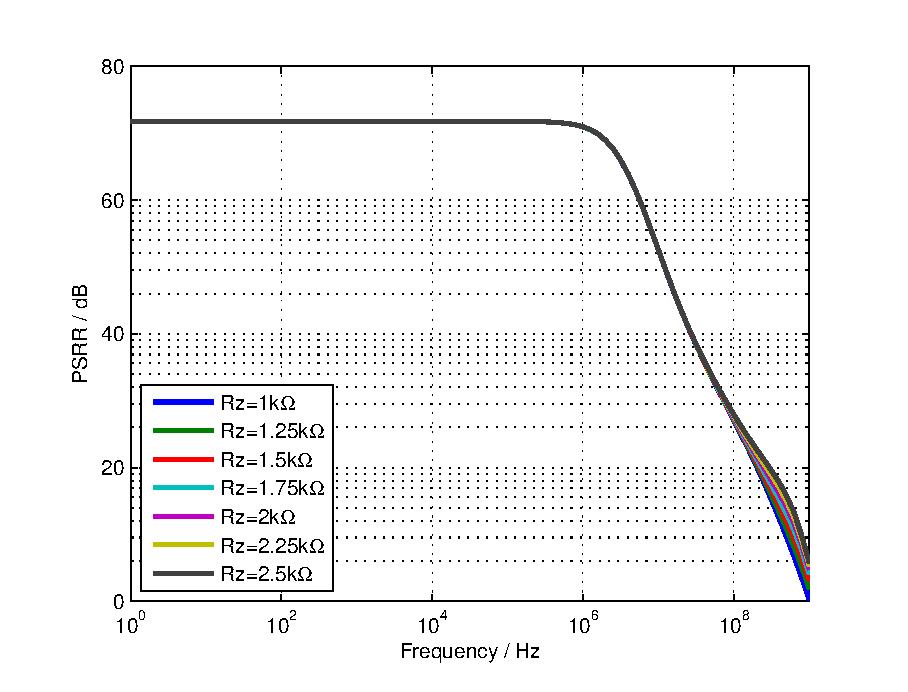
\includegraphics[width=0.7\textwidth]{chap4/res/PSRR_Rz.eps}
	\bicaption[fig:psrrrz]{两级运放针的$PSRR$对调零电阻$R_z$的参数扫描结果}{两级运放针的$PSRR$对补偿电容$R_z$的参数扫描结果}{Fig}{Parameter sweep results for $PSRR$ of compensation capacitor $R_z$ in two-stage opamp}
\end{figure}

根据图\ref{fig:cmrrcc}至图\ref{fig:psrrrz}的结果,可以看到CMRR和PSRR在高频接近转角频率处对于补偿电容$C_c$的变化较为敏感;
然而在同样的区域调零电阻的影响相对小了很多。
根据这些信息,电路工程师可以更方便地观察不同元件取值的影响,从而更有效率地进行电路设计。

\subsection{敏感度方法进行电路参数优化共模电源抑制比}
\label{subsec:cmps:test:sens}

最后,我们对CMRR和PSRR的敏感度进行计算,并尝试通过敏感度进行电路优化。
这里仍然针对两级运放进行分析,我们对其中的第一级和第二级的输入MOS管$M_1$和$M_6$的尺寸求取敏感度。
相应的敏感度结果在图\ref{fig:SensW6}和图\ref{fig:SensW6}中展现。

\begin{figure}[!htp]
	\centering
	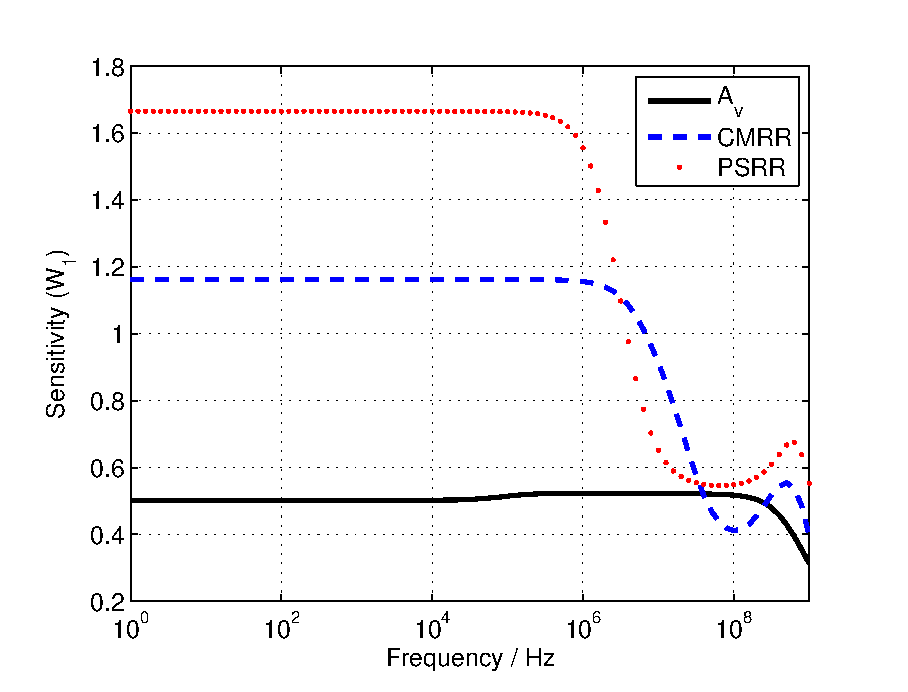
\includegraphics[width=0.7\textwidth]{chap4/res/SensW1.eps}
	\bicaption[fig:SensW1]{两级运放针对$W_1$的敏感度分析结果}{两级运放针对$W_1$的敏感度分析结果}{Fig}{Sensitivity results of $W_1$ in two-stage opamp}
\end{figure}

\begin{figure}[!htp]
	\centering
	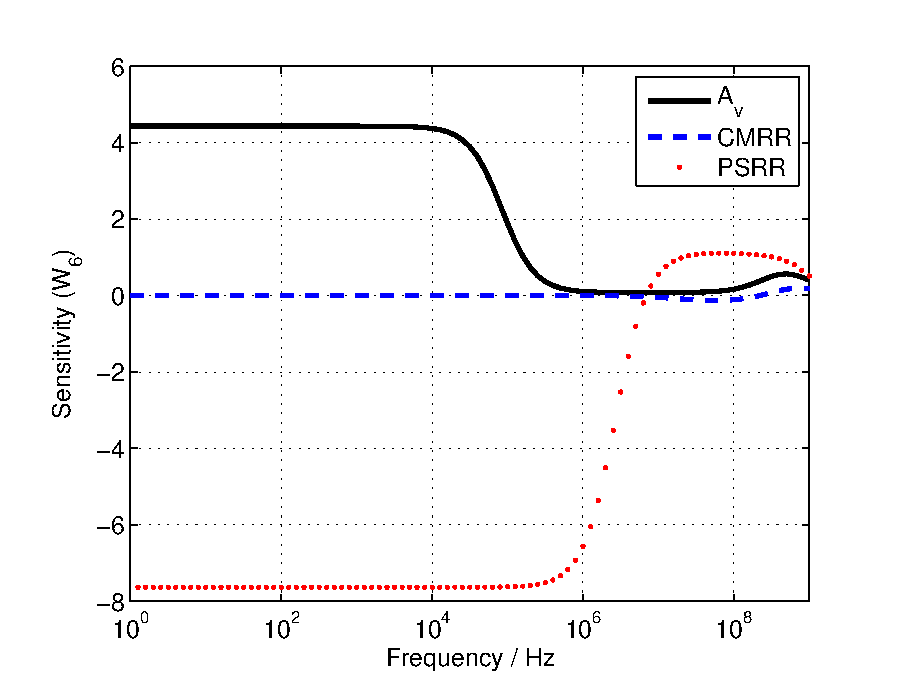
\includegraphics[width=0.7\textwidth]{chap4/res/SensW6.eps}
	\bicaption[fig:SensW6]{两级运放针对$W_6$的敏感度分析结果}{两级运放针对$W_6$的敏感度分析结果}{Fig}{Sensitivity results of $W_6$ in two-stage opamp}
\end{figure}

根据图中所展现的结果,我们看到$W_1$与三种电路指标$A_v$、$CMRR$和$PSRR$均正相关,故增大$W_1$将同时增大三种性能指标。
然而$W_6$情况则不同,如增大$W_6$的话,差分增益$A_v$会有所提升,$CMRR$基本保持不变,而$PSRR$则会下降。

我们在实际对运放进行了尺寸优化($W_1$从原有的$20\mu m$变为$30\mu m$,$W_6$从原有的$30\mu m$变为$31\mu m$)后,将相应的数据变化记录于表\ref{tab:sensw1}和表\ref{tab:sensw6}中。

\begin{table}[!htp]
	\bicaption[tab:sensw1]{$W_1$的DC敏感度分析结果及优化}{$W_1$的DC敏感度分析结果及优化}{Table}{Sensitivity analysis at DC of $W_1$}
	\centering
	\begin{tabular}{c|c|c|c|c|c}
		\hline
		\multirow{2}{*}{指标} & \multicolumn{2}{c|}{$W_1=20\mu m$} & \multicolumn{2}{c|}{$W_1=30\mu m$} & \multirow{2}{*}{比率} \\ \cline{2-5}
		                    &       值        &        敏感度        &       值        &        敏感度        &  \\ \hline
		       $A_v$        & 2.84K (69.1dB) &       0.502       & 3.41K (70.7dB) &       0.401       &  +20.0\% (+1.6dB)   \\ \hline
		      $CMRR$        & 2.07K (66.3dB) &       1.162       & 3.05K (69.7dB) &       0.802       &  +47.3\% (+3.4dB)   \\ \hline
		      $PSRR$        & 3.87K (71.8dB) &       1.665       & 6.92K (76.8dB) &       1.237       &  +78.8\% (+5.0dB)   \\ \hline
	\end{tabular}
\end{table}

\begin{table}[!htp]
	\bicaption[tab:sensw6]{$W_6$的DC敏感度分析结果及优化}{$W_6$的DC敏感度分析结果及优化}{Table}{Sensitivity analysis at DC of $W_6$}
	\centering
	\begin{tabular}{c|c|c|c|c|c}
		\hline
		\multirow{2}{*}{指标} & \multicolumn{2}{c|}{$W_6=30\mu m$} & \multicolumn{2}{c|}{$W_6=31\mu m$} & \multirow{2}{*}{比率} \\ \cline{2-5}
		                    &       值        &        敏感度        &       值        &        敏感度        &  \\ \hline
		       $A_v$        & 2.84K (69.1dB) &       4.43        & 3.04K (69.7dB) &       -0.20       &  +7.04\% (+0.6dB)   \\ \hline
		      $CMRR$        & 2.07K (66.3dB) &      6.1e-8       & 2.07K (66.3dB) &      9.4e-8       &     +0\% (+0dB)     \\ \hline
		      $PSRR$        & 3.87K (71.8dB) &       -7.63       & 3.32K (70.4dB) &       -2.83       &  -14.2\% (-1.4dB)   \\ \hline
	\end{tabular}
\end{table}

可以看到在尺寸调整后,三种电路指标$A_v$、$CMRR$和$PSRR$均按预期发生了变化。
同时由于敏感度的定义,即可知道电路性能变化比率与敏感度基本成正比,这在表中的数据也得到了相应的验证。
高敏感度带来了更快的性能增长。
另外,还应观察到在电路尺寸改变后电路的敏感度也发生了变化。
例如,表\ref{tab:sensw6}中的有关$A_v$的敏感度已经由正值变为了负值,说明继续增大$W_6$将对电路的增益带来不好的效果。

\section{本章小结}
\label{sec:cmps:con}

本章首先对GPDD多端口构造的方法的适用性条件进行了说明,并通过介绍$CMRR$和$PSRR$的计算,给出了具体的GPDD结构使用方法。
接着我们对GPDD中的敏感度分析方法进行了介绍。
最后,通过GPDD构造的高效性,参数扫描分析以及敏感性分析辅助电路优化等测试证明了这种构造方法的有效性。